\documentclass[final, pt]{beamer}

\usepackage[size=a1,orientation=landscape, scale=1.3]{beamerposter}

\usepackage{adjustbox}
\usepackage{caption}
\usepackage{enumitem}
\usepackage{graphicx}
\usepackage{lipsum}
\usepackage{pgfmath}
\usepackage{pgfplots}
\usepackage{ragged2e}
\usepackage{subcaption}
\usepackage{tikz}
\usepackage{transparent}

\usetikzlibrary{arrows.meta}
\usetikzlibrary{calc}

% Define the theme
\usetheme{metropolis}

% Colours
\definecolor{uiored}{HTML}{DD0000}
\definecolor{uiogrey}{HTML}{B2B3B7}
\definecolor{uioblack}{HTML}{000000}
\definecolor{uiowhite}{HTML}{FFFFFF}

% Define the colors
\definecolor{background}{HTML}{FAFAFA}
\setbeamercolor{block title}{bg=background,fg=red}
\setbeamercolor{block body}{bg=background,fg=black}
\setbeamercolor{title}{bg=uiored,fg=uiowhite}
\setbeamercolor{authors}{bg=uioblack,fg=uiowhite}

\setbeamertemplate{page number}{}
\setlength{\paperwidth}{\textwidth}
\setbeamersize{text margin left=0pt, text margin right=0pt}

% Title and author information
\title{\Huge{Enhancing the sensitivity of brain age models with explainable artificial intelligence}}


\definecolor{cb-green}{HTML}{4dac93}
\definecolor{cb-blue}{HTML}{3594d6}

\def\verticalspace{0.61cm}

\captionsetup[figure]{labelformat=empty}

\begin{document}

\newcommand{\convside}[6]{
    \node[
        fill=#5,
        inner sep=0pt,
        outer sep=0pt,
        minimum width=#3,
        minimum height=#4,
        draw=black
    ] (#6) at (#1, #2) {};
}

\newcommand{\convtop}[4]{
    \draw[fill=#4] #1 --
    ($ #1 + (#3, #3) $) --
    ($ #1 + (#3+#2, #3) $) --
    ($ #1 + (#2, 0) $);
}

\newcommand{\convfront}[3]{
    \draw[black, fill=#3] #1 --
                         ($ #1 + (1*#2, 1*#2) $) --
                         ($ #1 + (1*#2, 1*#2 - 2*#2) $) --
                         ($ #1 + (0, -2*#2) $);
}


\newcommand{\convchannel}[5]{
    \def\huemin{20}
    \def\huemax{80}
    \pgfmathsetmacro{\iterations}{#5-1}
    \foreach \i in {0,...,\iterations} {
        \pgfmathsetmacro{\hue}{int(random(\huemin, \huemax))}
        \convside{#1}{#2+\i*-3/3}{#3}{#4/#5}{black!\hue}{n\i0}
        \convtop{($ (n00.north west) + (0.5*\i*#4/#5, 0.5*\i*#4/#5) $)}{#3}{0.5*#4/#5}{black!\hue}

        \foreach \j in {0,...,\iterations} {
            \pgfmathsetmacro{\innerhue}{int(random(\huemin, \huemax))}
            \ifnum\j=0
                \pgfmathsetmacro{\innerhue}{\hue}
            \fi
            \convfront{($ (n00.north east) + (0.5*\j*#4/#5, 0.5*\j*#4/#5 - \i*#4/#5) $)}{0.5*#4/#5}{black!\innerhue}
        }
    }
}

\newcommand{\convlayer}[6]{
    \pgfmathsetmacro{\iterations}{#6-1}
    \foreach \i in {0,...,\iterations}{
        \pgfmathsetmacro{\x}{#1 + \i * 0.33}
        \convchannel{\x}{#2}{#3}{#4}{#5}
    }
}

\newcommand{\cnnarrow}[2]{
    \draw[-stealth, line width=5pt, opacity=0.5] #1 -- #2;
}

\newcommand{\cnn}[2]{
    \cnnarrow{(#1 - 5, #2 - 1)}{(#1+0.5, #2 - 1)}
    \convlayer{#1}{#2}{0.33cm}{6cm}{6}{3}
    \cnnarrow{(#1 + 2.325, #2 - 1)}{(#1+5.5, #2 - 1)}
    \convlayer{#1 + 5}{#2-0.5}{0.33cm}{4cm}{4}{5}
    \cnnarrow{(#1 + 7.5, #2 - 1)}{(#1+10, #2 - 1)}
    \convlayer{#1 + 9.6}{#2-1}{0.33cm}{2cm}{2}{7}
    \cnnarrow{(#1 + 12.25, #2 - 1)}{(#1+14.5, #2 - 1)}
    \draw[thick, dashed] (#1 - 0.8, #2 + 4) --
                         (#1 + 13.3, #2 + 4) --
                         (#1 + 13.3, #2 - 6) --
                         (#1 - 0.8, #2 - 6) -- cycle;
    \node[anchor=south] at (#1 + 6.35, #2 + 4) {
        \textbf{\large{Convolutional neural network}}
    };
}

\newcommand{\lrp}[2]{
    \cnnarrow{(#1 - 2.5, #2 - 1)}{(#1+0.5, #2 - 1)}
    \convlayer{#1}{#2-1}{0.33cm}{2cm}{2}{7}
    \convlayer{#1 + 4.3}{#2-0.5}{0.33cm}{4cm}{4}{5}
    \convlayer{#1 + 9}{#2}{0.33cm}{6cm}{6}{3}
    \draw[thick, dashed] (#1 - 0.8, #2 + 4) --
                         (#1 + 13.3, #2 + 4) --
                         (#1 + 13.3, #2 - 6) --
                         (#1 - 0.8, #2 - 6) -- cycle;
    \node[anchor=north] at (#1 + 6.35, #2 - 6) {
        \textbf{\large{Layerwise relevance propagation}}
    };
}

\newsavebox{\overview}
\sbox{\overview}{%
    \def\nodesize{1cm}
    \def\predictfill{blue}
    \begin{tikzpicture}
        \node[draw=black] at (0, 0) {};
        \node[draw=black] at (55, -25) {};
        \node[yslant=1] at (5, -7.5) {
            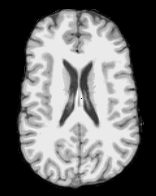
\includegraphics[height=5cm]{data/bert.png}
        };
        \node[] at (50, -7.5) {
            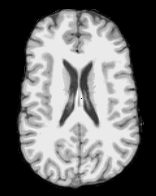
\includegraphics[height=7cm]{data/bert.png}
        };
        \node[align=center,font=\Large, text depth=0] at (27.5, -7.5) {
            Predicted\\brain age
        };

        %\convlayer{10}{-7.5}{1cm}{7cm}{7}{3}
        \cnn{10}{-6.5}
        \lrp{33}{-6.5}
        % \fiveconvlayer{15}{-7.5}{3cm}{5cm}{5}{5}
        % \sevenconvlayer{20}{-7.5}{5cm}{3cm}{3}{7}
    \end{tikzpicture}
}

% Start the poster
\begin{frame}[t]
    \thispagestyle{empty}

% Title and author block
    \begin{beamercolorbox}[sep=0em,wd=\textwidth]{title}
        \centering\\[4cm]
        \fontsize{48}{48}{\textbf{\inserttitle}}\\[3.25cm]

    \end{beamercolorbox}

    \begin{beamercolorbox}[sep=0em, wd=\textwidth]{authors}
        \def\authorwidth{.16\textwidth}
        \begin{columns}[T]
            \begin{column}{\authorwidth}
                \centering
                Esten H. Leonardsen\\
                University of Oslo\\
                \vspace{1em}
            \end{column}
            \begin{column}{\authorwidth}
                \centering
                Yunpeng Wang\\
                University of Oslo
            \end{column}
            \begin{column}{\authorwidth}
                \centering
                Lars T. Westlye\\
                University of Oslo
            \end{column}
            \begin{column}{\authorwidth}
                \centering
                Thomas Wolfers\\
                University of Tübingen
            \end{column}
        \end{columns}
    \end{beamercolorbox}

    \begin{columns}[t]
        \begin{column}{0.32\textwidth}
            \lipsum[1-4]
        \end{column}
        \begin{column}{0.66\textwidth}
            %\usebox{\overview}
        \end{column}
    \end{columns}

    \vfill
    \begin{beamercolorbox}[sep=0pt,wd=\textwidth]{title}
        \centering
        \begin{tikzpicture}
            \node[] at (0, 0) {
                
\includegraphics[height=3cm]{data/uio.png}
            };
        \end{tikzpicture}
    \end{beamercolorbox}


\end{frame}

\end{document}
